% Documento principal. Overleaf: selecionar main.tex e compilar com pdfLaTeX.
% Para revisão cega, selecionar submissao_cega.tex.
\documentclass[12pt,a4paper]{article}
\usepackage[T1]{fontenc}
\usepackage[utf8]{inputenc}
\usepackage[spanish,english,brazil]{babel}
\usepackage{newtxtext,newtxmath}
\usepackage[margin=2.5cm]{geometry}
\usepackage{graphicx,booktabs,tabularx,array,amsmath,longtable}
\usepackage{setspace,indentfirst,microtype}
\usepackage[round,authoryear,semicolon,sort]{natbib}
\usepackage{caption,placeins}
\usepackage{xurl}
\usepackage[hidelinks,unicode]{hyperref}
\hypersetup{pdfauthor={},pdftitle={Material Suplementar S1: simulações da CMMA}}
\setlength{\parindent}{1.25cm}
\setlength{\parskip}{0pt}
\setstretch{1.15}
\setlength{\emergencystretch}{2em}
\captionsetup{font=small,labelfont=bf,labelsep=period,justification=justified,singlelinecheck=false}
\setlength{\bibsep}{0.7\baselineskip}
\renewcommand{\bibsection}{\section*{Referências}}
\renewcommand{\bibfont}{\small\singlespacing\raggedright}
\newcommand{\fonte}[1]{\par\smallskip{\footnotesize\raggedright #1\par}}
\newcommand{\tituloPT}{Modelagem dos manguezais da costa macrotidal da Amazônia sob cenários de elevação do nível do mar até o final do século XXI}

\renewcommand{\thesection}{S\arabic{section}}
\renewcommand{\theequation}{S\arabic{equation}}
\renewcommand{\thetable}{S\arabic{table}}
\renewcommand{\thefigure}{S\arabic{figure}}
\begin{document}
\begin{center}{\Large\bfseries Material Suplementar S1\par}\medskip
\tituloPT
\end{center}
\section{Inventário e rastreabilidade}
Este Material Suplementar S1 documenta os cálculos e a configuração das simulações SSP1-2.6, SSP2-4.5 e SSP5-8.5, entre 2025 e 2100. Os números de tabelas e equações recebem o prefixo S. O inventário municipal completo corresponde à Tabela S1, distribuída em \path{municipios_manguezais_cmma_2025.xlsx} e CSV, com totais por estado e recorte em arquivo complementar. O método utiliza o centro dos pixels e conserva uma categoria sem correspondência municipal \citep{ibge2025,dados2026}. As áreas se restringem ao recorte, sem extrapolação para o território integral dos municípios.

A estatística oficial da Coleção 11 registra 10.436,2895 km$^2$ de manguezais no Brasil em 2025; o recorte de 6.782,8977 km$^2$ representa 64,99\% do total nacional \citep{mapbiomasareas2026}. A cobertura do recorte totaliza 6.782,8977 km$^2$: 2.241,0297 no Pará, 4.509,4455 no Maranhão e 32,4225 sem atribuição municipal. A máscara com elevação válida reduz esse total a 6.758,8650 km$^2$: 2.229,1992 no Pará, 4.504,6215 no Maranhão e 25,0443 sem atribuição. A diferença de 24,0327 km$^2$ decorre da cobertura altimétrica disponível. A planilha enumera 26 municípios paraenses e 39 maranhenses.

Os resultados analisados correspondem às execuções \path{run_20261021T034907} (SSP1-2.6), \path{run_20261021T113825} (SSP2-4.5) e \path{run_20261021T223331} (SSP5-8.5). Os metadados, as forçantes aplicadas e as trajetórias de estado estão nas subpastas dos cenários. O ensaio anterior com classes personalizadas não integra este artigo. O arquivo \path{MANIFESTO_ARQUIVOS.json} conserva a identificação e os resumos criptográficos dos arquivos preparados; não constitui um manifesto do presente pacote editorial.

\section{Classes, domínio e atualização}
A grade contém 18.415 linhas e 21.292 colunas, com 77.061.011 células válidas de 900 m$^2$. A Tabela S2 apresenta os códigos da Coleção 11 do MapBiomas \citep{mapbiomas2026} e o agrupamento aplicado. As escolhas de bloqueio e agrupamento são condições do experimento.
\setcounter{table}{1}
\begin{table}[htbp]\centering\small
\caption{Correspondência entre cobertura inicial e classes de entrada.}
\begin{tabularx}{\linewidth}{rXl}\toprule
Código & Categoria MapBiomas & Classe do modelo\\\midrule
3 & Formação Florestal & Vegetação natural \\
4 & Formação Savânica & Vegetação natural \\
5 & Mangue & Manguezal \\
6 & Floresta Alagável & Vegetação natural \\
9 & Silvicultura & Área antropizada \\
11 & Campo Alagado e Área Pantanosa & Vegetação natural \\
12 & Formação Campestre & Vegetação natural \\
15 & Pastagem & Área antropizada \\
21 & Mosaico de usos & Área antropizada \\
23 & Praia, Duna e Areal & Área bloqueada \\
24 & Área Urbanizada & Área antropizada \\
25 & Outras Áreas não Vegetadas & Área antropizada \\
30 & Mineração & Área antropizada \\
31 & Aquicultura & Área antropizada \\
32 & Apicum & Área bloqueada \\
33 & Rio, Lago e Oceano & Água \\
35 & Dendê & Área antropizada \\
39 & Soja & Área antropizada \\
41 & Outras Lavouras Temporárias & Área antropizada \\
50 & Restinga Herbácea ou Arbustiva & Vegetação natural \\
\bottomrule\end{tabularx}
\fonte{Fonte: legenda MapBiomas e configuração das execuções. O CSV inclui contagens e áreas iniciais por código.}
\end{table}

O catálogo de saída utiliza os códigos: 1, área antropizada; 2, área bloqueada; 3, manguezal; 4, vegetação natural; 5, água; 6, área antropizada inundada; 7, área bloqueada inundada; 8, manguezal inundado; 9, vegetação natural inundada; 10, manguezal migrado. A inundação de uma área bloqueada não a torna elegível à migração.

A sequência de atualização é descrita a partir da implementação arquivada, para explicitar os procedimentos efetivamente utilizados \citep{studio2026}. No início de cada ano são copiadas as matrizes de estados, elevação e idade. Para uma célula de água ou inundada cuja elevação anterior é não negativa, identificam-se os vizinhos de menor elevação. O incremento anual do nível do mar, $\delta L_t$, em metros, é dividido entre a célula de origem $i$ e os vizinhos de menor elevação:
\begin{equation}
q_{i,t}=\frac{\delta L_t}{1+n_{i,t}^{-}},
\label{eq:fluxo}
\end{equation}
em que $t$ indica o ano, $i$ a célula de origem, $n_{i,t}^{-}$ o número de vizinhos com cota inferior no início do passo e $q_{i,t}$ a parcela, em metros, aplicada à célula de origem e a cada um desses vizinhos. Assim, a soma dos acréscimos atribuídos por uma célula de origem equivale ao incremento anual $\delta L_t$. Vizinhos com classe básica passível de inundação também recebem o estado inundado correspondente. A Equação~\ref{eq:fluxo} transcreve a regra computacional do BR-MANGUE Studio 1.4.4, conforme o código arquivado \citep{studio2026}; é uma regra discreta do modelo, não uma equação hidrodinâmica nem uma formulação atribuída a Bezerra et al.\ \citeyearpar{bezerra2014}. O artigo de Bezerra et al. fundamenta o antecedente da abordagem de autômatos celulares em manguezais. O limite de maré descrito a seguir participa da elegibilidade para migração.

Após essa operação, as células de manguezal inicial e as células migradas com idade funcional mínima de três anos podem converter vizinhos de vegetação natural em mangue migrado, quando a elevação corrente desses vizinhos é menor ou igual a $T+L_t$. Nessa expressão, $T$ é a referência operacional de maré e $L_t$ a elevação acumulada do nível do mar desde 2025, ambas em metros. A idade da nova célula é iniciada em zero. A regra de migração consulta os valores correntes durante a varredura da grade; a propagação da inundação utiliza os valores copiados no início do ano. Portanto, o processamento combina referências temporais distintas, conforme a ordem de atualização implementada.

Ao final do processamento anual de cada célula elegível, a acreção acrescenta 0,0024 m (2,4 mm) à sua cota. O fator 0,001 converte milímetros para metros; a operação representa a aplicação, uma vez por ano, da taxa uniforme de 2,4 mm ano$^{-1}$ estimada na compilação da Seção S5. Essa operação abrange os estados com comportamento de mangue, inclusive mangue inundado e migrado. Trata-se de um acréscimo paramétrico à elevação armazenada, sem simulação explícita de transporte ou balanço de massa de sedimentos. O estado migrado não apresenta transição posterior para inundação na versão aplicada. Consequentemente, sua área é cumulativa ao longo das simulações. As regras são idênticas nos três cenários e não são calibradas com os resultados produzidos.


A varredura percorre células válidas em ordem de linha e coluna. A migração consulta o estado corrente; a idade usada para reconhecer fontes migradas é a do início do passo. As células recém-migradas começam com idade zero. A condição altimétrica da propagação usa o valor da célula fonte e diferenças locais; a referência de maré atua na elegibilidade para migração. A inicialização conserva as cotas do ANADEM, sem subtrair 3,01 m de todo o terreno. Esses detalhes procedem das funções de atualização do motor e da preparação raster na versão 1.4.4 \citep{studio2026}.

\section{Projeções e interpolação}
Os arquivos \path{native_grid_locations_cmma.csv} e \path{native_cell_values_ssp126_p50.csv}, com equivalentes para os demais cenários, documentam os nove pontos e os valores usados. A seleção retém centros da grade regular do IPCC internos ao polígono, excluindo estações adicionais. As projeções são as de confiança média, percentil 50, versão 20210809 \citep{garner2021,fox2021,kopp2023}.

Para cada ponto, interpola-se linearmente o valor de 2025 e subtrai-se esse valor de todos os nós temporais. Calcula-se a mediana das nove diferenças em cada nó. O arquivo de entrada contém esses nós; o modelo interpola entre eles. A forçante anual é a diferença entre valores acumulados consecutivos. A presença de uma linha de 2020 no arquivo não muda o início da execução em 2025. Os arquivos \path{sea_level_forcing.csv} de cada cenário conservam os valores efetivamente aplicados.

Para dois nós consecutivos, $t_a$ e $t_b$, a interpolação emprega:
\begin{equation}
D_s(t)=D_s(t_a)+\frac{t-t_a}{t_b-t_a}\left[D_s(t_b)-D_s(t_a)\right].
\label{eq:interpolacao}
\end{equation}
Nessa expressão, $D_s(t)$ é a elevação acumulada interpolada no ano $t$, e $D_s(t_a)$ e $D_s(t_b)$ são os valores nos nós anterior e posterior; o fator $(t-t_a)/(t_b-t_a)$ determina a posição temporal entre eles. Esta é a expressão da interpolação linear implementada no processamento e no leitor de trajetórias \citep{studio2026}, aplicada aos dados de Garner et al.\ \citeyearpar{garner2021}. A divisão por 1.000 converte milímetros em metros. As elevações finais são 375,5, 508,5 e 712,5 mm; os incrementos iniciais de 2026 são 4,8, 4,7 e 5,0 mm, respectivamente. Não se calculam tendências observadas contemporâneas a partir dessas projeções.

\section{Referência operacional de maré}
A Tabela S3 conserva os máximos e níveis médios das oito tábuas de 2026 \citep{chm2026}. $H_{\max}$ e $NM$ usam o nível de redução (NR) próprio de cada estação. A subtração dentro de cada tábua elimina esse deslocamento local; não resolve a diferença de nível médio entre estações.
\begin{table}[htbp]\centering\small
\caption{Síntese das tábuas de marés de 2026; valores em metros.}
\begin{tabularx}{\linewidth}{Xrrr}\toprule
Estação & $H_{\max}$ sobre NR & $NM$ sobre NR & $H_{\max}-NM$\\\midrule
Ilha dos Guarás & 5,43 & 2,74 & 2,69\\
Fundeadouro de Salinópolis & 5,41 & 2,75 & 2,66\\
Ilha do Mosqueiro & 3,87 & 1,95 & 1,92\\
Porto de Belém & 3,60 & 1,75 & 1,85\\
São Luís & 6,17 & 3,27 & 2,90\\
Terminal da Ponta da Madeira & 6,17 & 3,23 & 2,94\\
Porto de Itaqui & 6,70 & 3,40 & 3,30\\
Terminal da Alumar & 6,57 & 3,42 & 3,15\\
\bottomrule\end{tabularx}
\fonte{Fonte: CHM (2026), processamento das tábuas. A média da última coluna é 2,67625 m; a mediana é 2,795 m.}
\end{table}
A vinculação vertical disponível para Itaqui utiliza a altitude elipsoidal da RN2 ($h=-20,9017$ m), a ondulação geoidal EGM2008 ($N=-25,8265$ m) e a distância vertical entre a RN2 e o nível de redução ($d=7,996$ m), documentadas nas fichas e no cálculo geoidal \citep{chm2001,chm2018,karney}. A conversão $H=h-N$, seguida da subtração de $d$, fornece $NR_{EGM2008}=-3,0712$ m. Somado ao nível médio de Itaqui, de 3,40 m acima do NR, esse valor resulta em 0,3288 m. Adota-se então:
\begin{equation}
T=\frac{1}{8}\sum_{j=1}^{8}(H_{\max,j}-NM_j)+NM_{Itaqui,EGM2008}
  =2,67625+0,3288\simeq3,01\ \mathrm{m}.
\label{eq:mare}
\end{equation}
Na Equação~\ref{eq:mare}, $j$ identifica cada estação; $H_{\max,j}$ é a maior preamar prevista e $NM_j$ o nível médio informado na tábua, ambos relativos ao nível de redução local; $NM_{Itaqui,EGM2008}$ é o nível médio de Itaqui convertido ao EGM2008. A média dos oito valores de $H_{\max,j}-NM_j$ descreve quanto a maior preamar prevista supera o nível médio em cada estação. Somar a correção de Itaqui transfere essa referência para as cotas do ANADEM. A Equação~\ref{eq:mare} é uma aproximação definida neste estudo. Seu uso transfere a referência média de Itaqui ao recorte e atribui pesos iguais às estações, inclusive às concentradas no entorno de São Luís. A vinculação utiliza levantamento GNSS de 2001, com precisão vertical informada de 0,1196 m. Macromaré é classificada pela amplitude entre preamar e baixamar, com limite clássico acima de 4 m; para setores entre Pará e Maranhão, a literatura reporta 4--7,5 m \citep{davies1964,souzafilho2005}. O valor calculado de 3,01 m é um limiar altimétrico operacional relativo ao EGM2008, não uma amplitude nem uma taxa anual de elevação do mar, portanto não deve ser comparado ao critério de macromaré. A memória de cálculo e a transferência espacial permanecem documentadas aqui.


O arquivo \path{origem_calculo_mare.json} registra a ausência de um limiar absoluto regional geodeticamente determinado e, separadamente, a aproximação operacional de 3,01 m utilizada. O valor nulo do campo regional absoluto é intencional. A síntese não corresponde a uma maré simultânea, nem à média de todas as preamares. O DEM permanece em EGM2008, enquanto a referência mareal envolve a hipótese espacial descrita acima.

\section{Acreção e maturação funcional}
A Tabela S4 explicita os 20 valores da compilação. Passos et al.\ \citeyearpar{passos2023} apresentam testemunhos de manguezais de Mocajuba/Curuçá, com cronologia por excesso de $^{210}$Pb. Lacerda et al.\ \citeyearpar{lacerda2024}, Tabela 4, compilam valores de Marajó para posições de mangue baixo (LM) e alto (UM), igualmente derivados de $^{210}$Pb. Os valores de Marajó são citados pela compilação consultada, sem atribuição de coleta aos autores deste artigo.
\begin{table}[htbp]\centering\small
\caption{Taxas de acreção que fundamentam o parâmetro uniforme.}
\begin{tabularx}{\linewidth}{Xll}\toprule
Origem/local & Taxas (mm ano$^{-1}$) & Referência\\\midrule
Mocajuba/Curuçá (4 testemunhos) & 1,9; 2,3; 2,3; 3,1 & Passos et al. (2023)\\
Afuá (LM; UM) & 1,4; 2,4 & Lacerda et al. (2024)\\
Breves (LM; UM) & 3,4; 2,2 & Lacerda et al. (2024)\\
Camará (LM; UM) & 1,4; 2,3 & Lacerda et al. (2024)\\
Chaves (LM; UM) & 2,4; 3,8 & Lacerda et al. (2024)\\
Jaranduba (LM; UM) & 2,3; 7,1 & Lacerda et al. (2024)\\
Pesqueira (LM; UM) & 1,7; 0,7 & Lacerda et al. (2024)\\
Ponta de Pedras (LM; UM) & 3,1; 3,5 & Lacerda et al. (2024)\\
São Sebastião (LM; UM) & 3,0; 3,8 & Lacerda et al. (2024)\\
\bottomrule\end{tabularx}
\fonte{Fontes: Passos et al. (2023) e compilação de Lacerda et al. (2024). São posições/testemunhos distintos, sem ponderação por área.}
\end{table}

A soma dos 20 valores é 54,2 mm ano$^{-1}$, resultando em média aritmética de 2,71 mm ano$^{-1}$. Os elementos centrais da série ordenada são 2,3 e 2,4; sua média fornece mediana de 2,35 mm ano$^{-1}$. Arredonda-se essa mediana a 2,4 mm ano$^{-1}$ para o parâmetro. A faixa é 0,7--7,1 mm ano$^{-1}$. Não se adicionam taxas de sedimentos subtidais de canais, máximos de zonas localizadas de convergência ou uma segunda síntese dos mesmos testemunhos. A concentração dos dados no Pará impede interpretar a mediana como estimativa espacialmente representativa da CMMA. A acreção é distinta da variação líquida da superfície \citep{woodroffe2016}.

A referência biológica utiliza \textit{Rhizophora mangle}, amplamente distribuída na costa estudada \citep{menezes2008}. Allen \citeyearpar{allen2002} relata início de floração por volta dos seis anos e possibilidade aos três a cinco. Dangremond e Feller \citeyearpar{dangremond2016} demonstram reprodução precoce e variação entre populações da Flórida. Não se dispõe de idade local de recrutamento calibrada para células de 30 m. Assim, adota-se o atraso de três anos como limite inferior operacional para que uma célula migrada passe a atuar como fonte de propágulos; o parâmetro é mantido constante entre cenários.

\section{Conferência e leitura dos indicadores}
A verificação reproduz as contagens dos rasters e as compara com as tabelas e os metadados, além de conferir máscara, códigos, alinhamento, sequência temporal, transições anuais e igualdade entre o estado final e a imagem de 2100. As trajetórias aplicadas são comparadas com os arquivos de entrada. Essa conferência estabelece a consistência dos arquivos e dos cálculos; a aplicação não inclui validação ecológica independente nem análise de sensibilidade dos parâmetros. As áreas representam medidas dos mapas classificados e simulados, sem ajuste por matriz de erro. A distinção em relação a estimativas de área corrigidas por acurácia segue Olofsson et al.\ \citeyearpar{olofsson2014}.

As figuras utilizam as contagens integrais e os rasters de estado. Para a comparação espacial detalhada, seleciona-se uma janela comum de 30 $\times$ 30 km com alta concentração conjunta de mangue inundado e migrado no SSP5-8.5, mediante busca em intervalos de 1,5 km. O enquadramento é mantido entre cenários. Essa seleção destaca um setor de mudança e não representa uma amostra probabilística da CMMA. As saídas de elevação ilustradas pela interface não integram a análise temporal, que utiliza exclusivamente estados e tabelas conferidos.


As identidades de área são formalizadas por:
\begin{equation}
A_{k,t}=n_{k,t}\times0,0009\ \mathrm{km}^{2},\qquad E_t=R_t+M_t,
\label{eq:area_supp}
\end{equation}
\begin{equation}
E_{2025}=R_t+I_t,\qquad C_t=100\frac{M_t}{I_t},
\label{eq:balance_supp}
\end{equation}
\begin{equation}
P_{j,t}=100\frac{M_{j,t}}{M_t},\qquad F_{j,t}=100\frac{M_{j,t}}{A_{j,2025}}.
\label{eq:origin_supp}
\end{equation}
Nessas expressões, $n_{k,t}$ é a contagem de células válidas na classe $k$ no ano $t$; $A_{k,t}$ é sua área; $R_t$ é o mangue da cobertura de 2025 que permanece; $I_t$ é a parcela dessa cobertura convertida para mangue inundado; $M_t$ é o mangue migrado; $E_t$ é a extensão total; $C_t$ é a compensação da área inundada pela migração; $M_{j,t}$ é a área migrada sobre a categoria inicial $j$; $P_{j,t}$ é sua participação no total migrado; e $F_{j,t}$ é a fração de sua área inicial convertida. A porcentagem de origem da migração usa $M_{2100}$ como denominador, enquanto a fração convertida usa a área inicial da categoria no domínio válido. Ambos os indicadores constam de \path{ORIGENS_MIGRACAO.csv}; a Figura S1 apresenta a distribuição de origens.

\begin{figure}[htbp]\centering
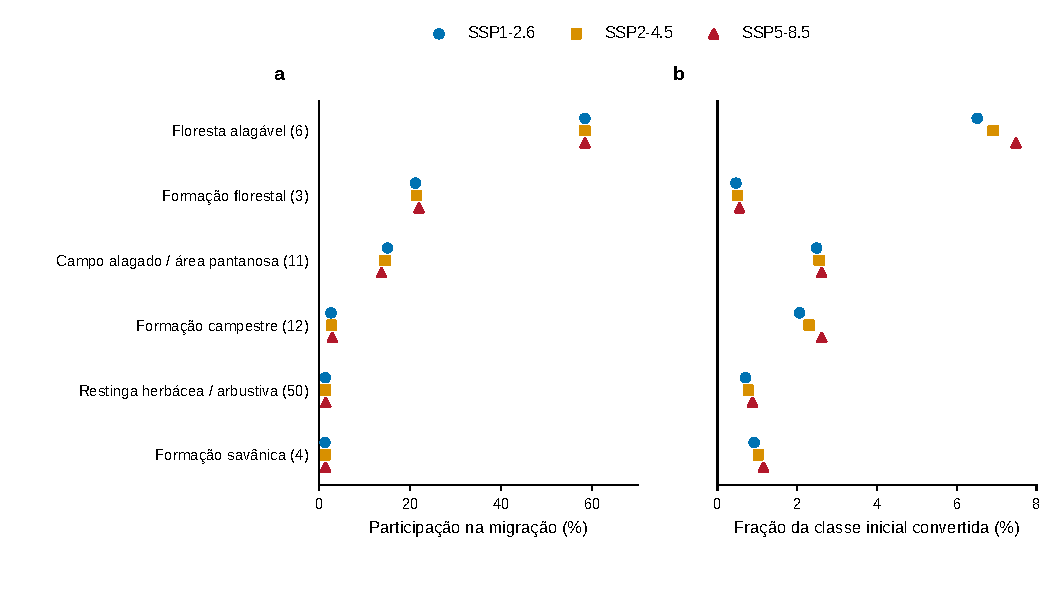
\includegraphics[width=\linewidth]{figuras/figura_s1.pdf}
\caption{Coberturas de 2025 que originam mangue migrado em 2100. (a) Participação de cada cobertura no total migrado de cada cenário. (b) Fração da área inicial de cada cobertura convertida em mangue migrado. Os painéis utilizam denominadores distintos.}
\fonte{Fontes: MapBiomas Coleção 11 e saídas conferidas das simulações.}
\end{figure}

As séries não incluem bandas de incerteza: cada cenário corresponde a uma execução determinística. O primeiro passo converte 182,4507 km$^2$ da cobertura inicial em mangue inundado nos três cenários. A ausência de controle com nível constante impede separar quantitativamente o ajuste inicial e a contribuição climática nessa resposta. A permanência do estado migrado e o bloqueio dos códigos 23 e 32 são condições conservadas na análise, sem alteração posterior das simulações.

\section{Desempenho e ambiente computacional}
As três execuções foram realizadas no mesmo computador: Intel Core i3-1215U, oito processadores lógicos, frequência máxima declarada de 4,4 GHz, 20,1 GB de memória DDR4-3200 e Ubuntu 26.04.1 LTS. Cada execução percorreu 77.061.011 células válidas em 75 passos anuais (5.779.575.825 operações célula-ano). O tempo registrado inicia após o carregamento dos rasters e a preparação do diretório, inclui o ciclo anual e a gravação de GeoTIFFs anuais, e não inclui a produção posterior de figuras, animações e relatórios. A taxa média é calculada como operações célula-ano divididas por esse tempo e, portanto, inclui o custo de gravação dos mapas. A métrica conta operações sobre células válidas, não mudanças efetivas de classe.

\setcounter{table}{4}
\begin{table}[htbp]\centering\small
\caption{Tempos e recursos registrados nas execuções analisadas.}
\begin{tabularx}{\linewidth}{lrrrr}
\toprule
Cenário & Tempo & Operações ($10^9$) & Operações s$^{-1}$ ($10^3$) & Pico RAM (GiB)\\
\midrule
SSP1-2.6 & 6:37:49 & 5,780 & 242,1 & 9,03\\
SSP2-4.5 & 6:45:58 & 5,780 & 237,3 & 9,00\\
SSP5-8.5 & 6:48:20 & 5,780 & 235,9 & 9,13\\
\bottomrule
\end{tabularx}
\fonte{Fonte: metadados das execuções \path{run_20261021T034907}, \path{run_20261021T113825} e \path{run_20261021T223331}, respectivamente.}
\end{table}

\FloatBarrier
\begin{thebibliography}{99}
\interlinepenalty=10000
\bibitem[Allen(2002)]{allen2002}
ALLEN, J. A. Rhizophora mangle L. In: VOZZO, J. A. (ed.). \textbf{Tropical tree seed manual}. Washington, DC: USDA Forest Service, 2002. p. 690--692. Disponível em: \url{https://www.fs.usda.gov/psw/publications/allen/psw_2002_allen009.pdf}.

\bibitem[Bezerra et~al.(2014)]{bezerra2014}
BEZERRA, D. da S. et al. Simulating sea-level rise impacts on mangrove ecosystem adjacent to anthropic areas: the case of Maranhão Island, Brazilian Northeast. \textbf{Pan-American Journal of Aquatic Sciences}, v. 9, n. 3, p. 188--198, 2014. Disponível em: \url{https://panamjas.org/pdf_artigos/PANAMJAS_9%283%29_188-198.pdf}.

\bibitem[Centro de Hidrografia da Marinha(2001)]{chm2001}
CENTRO DE HIDROGRAFIA DA MARINHA. \textbf{Ficha F-21: RN2, Porto de Itaqui}. Levantamento GNSS, 2001. Disponível em: \url{https://www.marinha.mil.br/chm/sites/www.marinha.mil.br.chm/files/anexo_topogeodesico/f-21-413-009-2001.pdf}.

\bibitem[Centro de Hidrografia da Marinha(2018)]{chm2018}
CENTRO DE HIDROGRAFIA DA MARINHA. \textbf{Ficha F-41: Porto de Itaqui, estação 30110}. 2018. Disponível em: \url{https://www.marinha.mil.br/chm/sites/www.marinha.mil.br.chm/files/dados_de_mare/30110_-_porto_de_itaqui_f-41_-_tabuas_padrao_v1-18.pdf}.

\bibitem[Centro de Hidrografia da Marinha(2026)]{chm2026}
CENTRO DE HIDROGRAFIA DA MARINHA. \textbf{Tábuas das Marés 2026}. Niterói: Marinha do Brasil, 2026. Disponível em: \url{https://www.marinha.mil.br/chm/tabuas-de-mare-6?page=0}.

\bibitem[Dangremond \& Feller(2016)]{dangremond2016}
DANGREMOND, E. M.; FELLER, I. C. Precocious reproduction increases at the leading edge of a mangrove range expansion. \textbf{Ecology and Evolution}, v. 6, p. 5087--5092, 2016. DOI: \url{https://doi.org/10.1002/ece3.2270}.

\bibitem[Davies(1964)]{davies1964}
DAVIES, J. L. A morphogenic approach to world shorelines. \textbf{Zeitschrift für Geomorphologie}, v. 8, n. 5, p. 127--142, 1964. DOI: \url{https://doi.org/10.1127/zfg/mortensen/8/1964/127}.

\bibitem[Fox-Kemper et~al.(2021)]{fox2021}
FOX-KEMPER, B. et al. Ocean, cryosphere and sea level change. In: MASSON-DELMOTTE, V. et al. (ed.). \textbf{Climate Change 2021: The Physical Science Basis}. Cambridge: Cambridge University Press, 2021. p. 1211--1362. DOI: \url{https://doi.org/10.1017/9781009157896.011}.

\bibitem[Garner et~al.(2021)]{garner2021}
GARNER, G. G. et al. \textbf{IPCC AR6 Sea Level Projections}. Versão 20210809. Zenodo, 2021. Conjunto de dados. DOI: \url{https://doi.org/10.5281/zenodo.6382554}.

\bibitem[IBGE(2025a)]{ibge2025}
IBGE. \textbf{Malha Municipal Digital 2025: Pará e Maranhão}. Rio de Janeiro: IBGE, 2025a. Disponível em: \url{https://geoftp.ibge.gov.br/organizacao_do_territorio/malhas_territoriais/malhas_municipais/municipio_2025/UFs/}.

\bibitem[Karney(s.d.)]{karney}
KARNEY, C. F. F. \textbf{GeographicLib: GeoidEval}. Documentação do cálculo de alturas geoidais. [S. l.], [s. d.]. Disponível em: \url{https://geographiclib.sourceforge.io/html/GeoidEval.1.html}.

\bibitem[Kopp et~al.(2023)]{kopp2023}
KOPP, R. E. et al. The Framework for Assessing Changes To Sea-level (FACTS) v1.0: a platform for characterizing parametric and structural uncertainty in future global, relative, and extreme sea-level change. \textbf{Geoscientific Model Development}, v. 16, p. 7461--7489, 2023. DOI: \url{https://doi.org/10.5194/gmd-16-7461-2023}.

\bibitem[Lacerda et~al.(2024)]{lacerda2024}
LACERDA, L. D. de; FERREIRA, A. C.; BORGES, R.; WARD, R. Challenges to mangroves of the Semiarid Equatorial Coast of Brazil in the Anthropocene. \textbf{Cambridge Prisms: Coastal Futures}, v. 2, e17, 2024. DOI: \url{https://doi.org/10.1017/cft.2024.16}.

\bibitem[MapBiomas(2026a)]{mapbiomas2026}
MAPBIOMAS. \textbf{Coleção 11: cobertura e uso da terra, 30 m, 1985--2025}. MapBiomas Brasil, 2026. Disponível em: \url{https://brasil.mapbiomas.org/iniciativas-e-produtos/cobertura-e-uso-da-terra/cobertura-30m/cobertura/}.

\bibitem[MapBiomas(2026b)]{mapbiomasareas2026}
MAPBIOMAS. \textbf{Coleção 11: área de cobertura e uso da terra por estado, 1985--2025}. MapBiomas Brasil, 2026. Planilha de estatísticas, classe Mangue, ano 2025. Disponível em: \url{https://brasil.mapbiomas.org/wp-content/uploads/sites/3/2026/08/MAPBIOMAS_BRAZIL-COL.11-BIOME_STATE.xlsx}.

\bibitem[Menezes et~al.(2008)]{menezes2008}
MENEZES, M. P. M. de; BERGER, U.; MEHLIG, U. Mangrove vegetation in Amazonia: a review of studies from the coast of Pará and Maranhão States, north Brazil. \textbf{Acta Amazonica}, v. 38, n. 3, p. 403--420, 2008. DOI: \url{https://doi.org/10.1590/S0044-59672008000300004}.

\bibitem[Olofsson et~al.(2014)]{olofsson2014}
OLOFSSON, P. et al. Good practices for estimating area and assessing accuracy of land change. \textbf{Remote Sensing of Environment}, v. 148, p. 42--57, 2014. DOI: \url{https://doi.org/10.1016/j.rse.2014.02.015}.

\bibitem[Passos et~al.(2023)]{passos2023}
PASSOS, T. et al. Low carbon accumulation in a macro-tidal mangrove forest on the Amazon coast. \textbf{Limnology and Oceanography}, v. 68, p. 1936--1948, 2023. DOI: \url{https://doi.org/10.1002/lno.12396}.

\bibitem[Sousa et~al.(2026a)]{studio2026}
SOUSA, F. M.; BEZERRA, D. da S.; COSTA, S. S.; SANTOS, R. L. \textbf{BR-MANGUE Studio}. Versão 1.4.4. Zenodo, 2026a. Software. DOI: \url{https://doi.org/10.5281/zenodo.23527116}.

\bibitem[Sousa et~al.(2026b)]{dados2026}
SOUSA, F. M.; BEZERRA, D. da S.; COSTA, S. S.; SANTOS, R. L. \textbf{Manguezais da CMMA por município -- 2025}. Versão a1a9aea. GitHub, 2026b. Conjunto de dados. Disponível em: \url{https://github.com/oceanpep/br-mangue-studio/tree/a1a9aea6a176e0bb177f088f8be3ec5932248e4d/datasets/cmma_municipalities_2025}.

\bibitem[Souza-Filho(2005)]{souzafilho2005}
SOUZA-FILHO, P. W. M. Costa de manguezais de macromaré da Amazônia: cenários morfológicos, mapeamento e quantificação de áreas usando dados de sensores remotos. \textbf{Revista Brasileira de Geofísica}, v. 23, n. 4, p. 427--435, 2005. DOI: \url{https://doi.org/10.1590/S0102-261X2005000400006}.

\bibitem[Woodroffe et~al.(2016)]{woodroffe2016}
WOODROFFE, C. D. et al. Mangrove sedimentation and response to relative sea-level rise. \textbf{Annual Review of Marine Science}, v. 8, p. 243--266, 2016. DOI: \url{https://doi.org/10.1146/annurev-marine-122414-034025}.

\end{thebibliography}
\end{document}
